\documentclass[12pt,letterpaper]{article}
\usepackage{amsmath}
\usepackage{amsfonts}
\usepackage{amssymb}
\usepackage{textcomp}
\usepackage{indentfirst}
\usepackage{hyperref}
\usepackage{graphicx}
\usepackage[margin=2.5cm]{geometry}

\usepackage{listings}
\lstset{language=bash, basicstyle=\footnotesize\ttfamily}

\author{Andrew Price}
\title{Kuka KR-5sixx 650WP System Configuration}
\begin{document}
\maketitle

Important configuration information the KR-5sixx in Henrik’s lab.

\section{Rotation Conventions}

Euler rotation angles reported by the robot are returned as angles A, B, and C. These angles are the rotations about the X, Y, and Z axes, respectively. However, the rotations are applied in the YPR order, the reverse of the order in which they appear in the XML protocol. To output coordinate frame is shown in Figure \ref{fig:flangeFrame}.
\begin{figure}[h!]
\centering
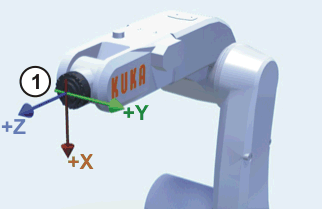
\includegraphics[scale=0.45]{tool_frame.png}
\caption{Kuka-defined flange coordinate frame. From \href{run:kr_5_sixx_wp_en.pdf}{``KR 5 sixx R650, R850 WP - Specification''}}
\label{fig:flangeFrame}
\end{figure}

\newpage
\section{Network Configuration}
\begin{figure}[h!]
\centering
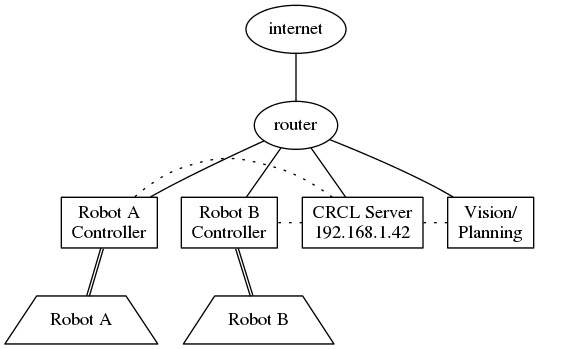
\includegraphics[scale=0.45]{network.png}
\caption{Data connections between robots, PCs, and network infrastructure.}
\label{fig:network}
\end{figure}
\section{Pneumatic System}
\subsection{Supply and Control Systems}
The air and vacuum supply lines are controlled from the compressor in CCB Room 322. See Dan with questions relating to their operation. A pressure regulator determines the actual system pressure in the robot arm.
\subsection{Runtime Operation}
Output pins are controlled over ERX via the \textbf{DiO} element. DiO contains bit flags for digital output pins, starting at \$OUT9. Pins \$OUT9-\$OUT15 control the pneumatic valve positions: to set Valve 1 to position A, \$OUT9 must be ON and \$OUT11 must be OFF, giving a DiO value of 05.

For more information on the ERX protocol, see the document \href{run:RSI_XML.pdf}{``KUKA.Ethernet RSI XML 1.1''}.

For more information on the pneumatic control valves, refer to the document \href{run:BA_KR_5_sixx_WP_en.pdf}{``KR 5 sixx R650, R850 WP - Operating Instructions''}.

\end{document}